\chapter{Methodology}
%%WHAT Is inference3
\label{chap:methodology}

In this section we present a methodology to create a decision model supporting the optimal selection of edge and cloud inference for real-time AI applications.
This methodology can be seen in figure \ref{fig:Methodology} and consists of a multi-step process, which this section will dissect into the individual steps.
%In this section we propose a methodology characterizing the deployment of deep learning models for inference, is presented.




\begin{figure}[H]
\centering
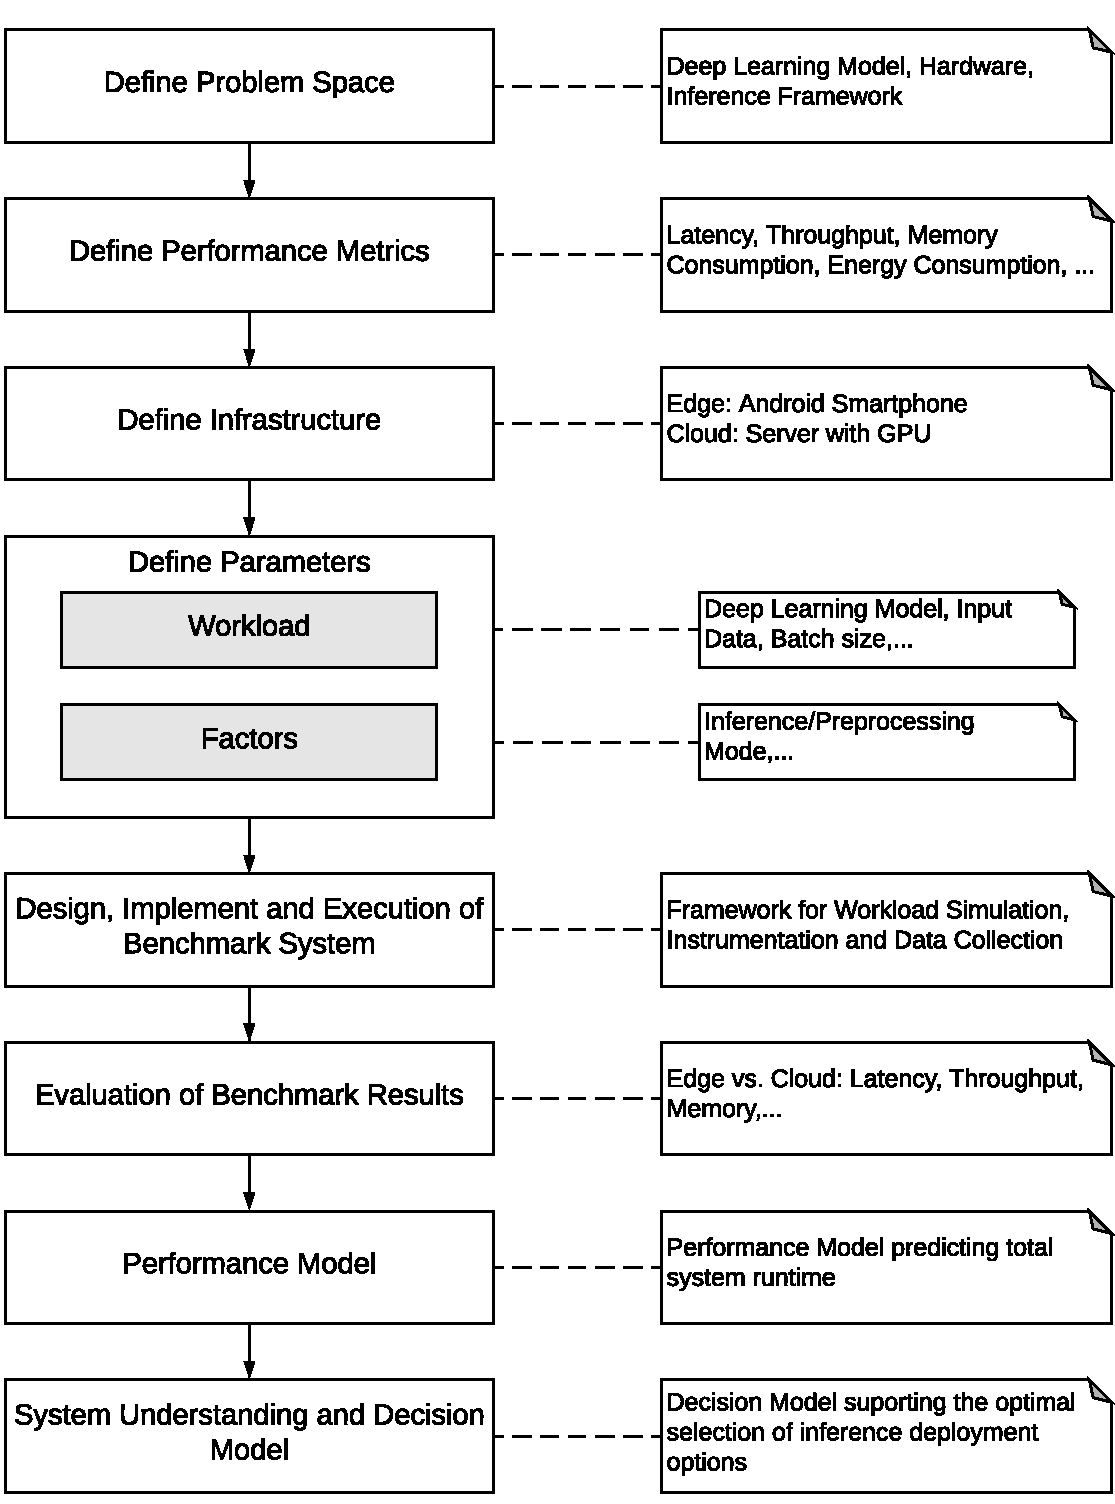
\includegraphics[width=0.9\textwidth]{./Bilder/Methodology.pdf}
\caption{Methodology to help with the optimal selection of cloud and edge inference for real-time AI}
\label{fig:Methodology}
\end{figure}


\section{Problem Space}
In order to model the performance of deep learning inference, it is crucial to understand the underlying problem space. 
In section \ref{chap:fundamentels} we presented the fundamentals of Deep Learning Models, their deployment and the frameworks needed to perform the inference.

\subsection{Deep Learning Model}
%architecture
%optimization
\subsection{Hardware}
\subsection{Inference Framework}
\begin{comment}



All aspects of the problem space hardware, model and the used inference framework have an impact on the performance, thus are the influencing factors on the inference performance.
In figure \ref{fig:perfmodel} we propose a performance model that takes all performance influencing factors as its inputs and maps them to performance metrics, which are essential for assessing inference performance for real-time AI applications.
These inputs affect various performance metrics, of which inference latency and throughput are the most important ones for real-time AI applications on the edge. However, as the hardware on edge devices is limited and most of the times more than one application needs to run in parallel, low usages of the other depicted metrics are vital as well.
In the following we present performance metrics essential for the performance of real-time AI applications and the rationale behind them.
\end{comment}
\begin{figure}[!htb]
\centering
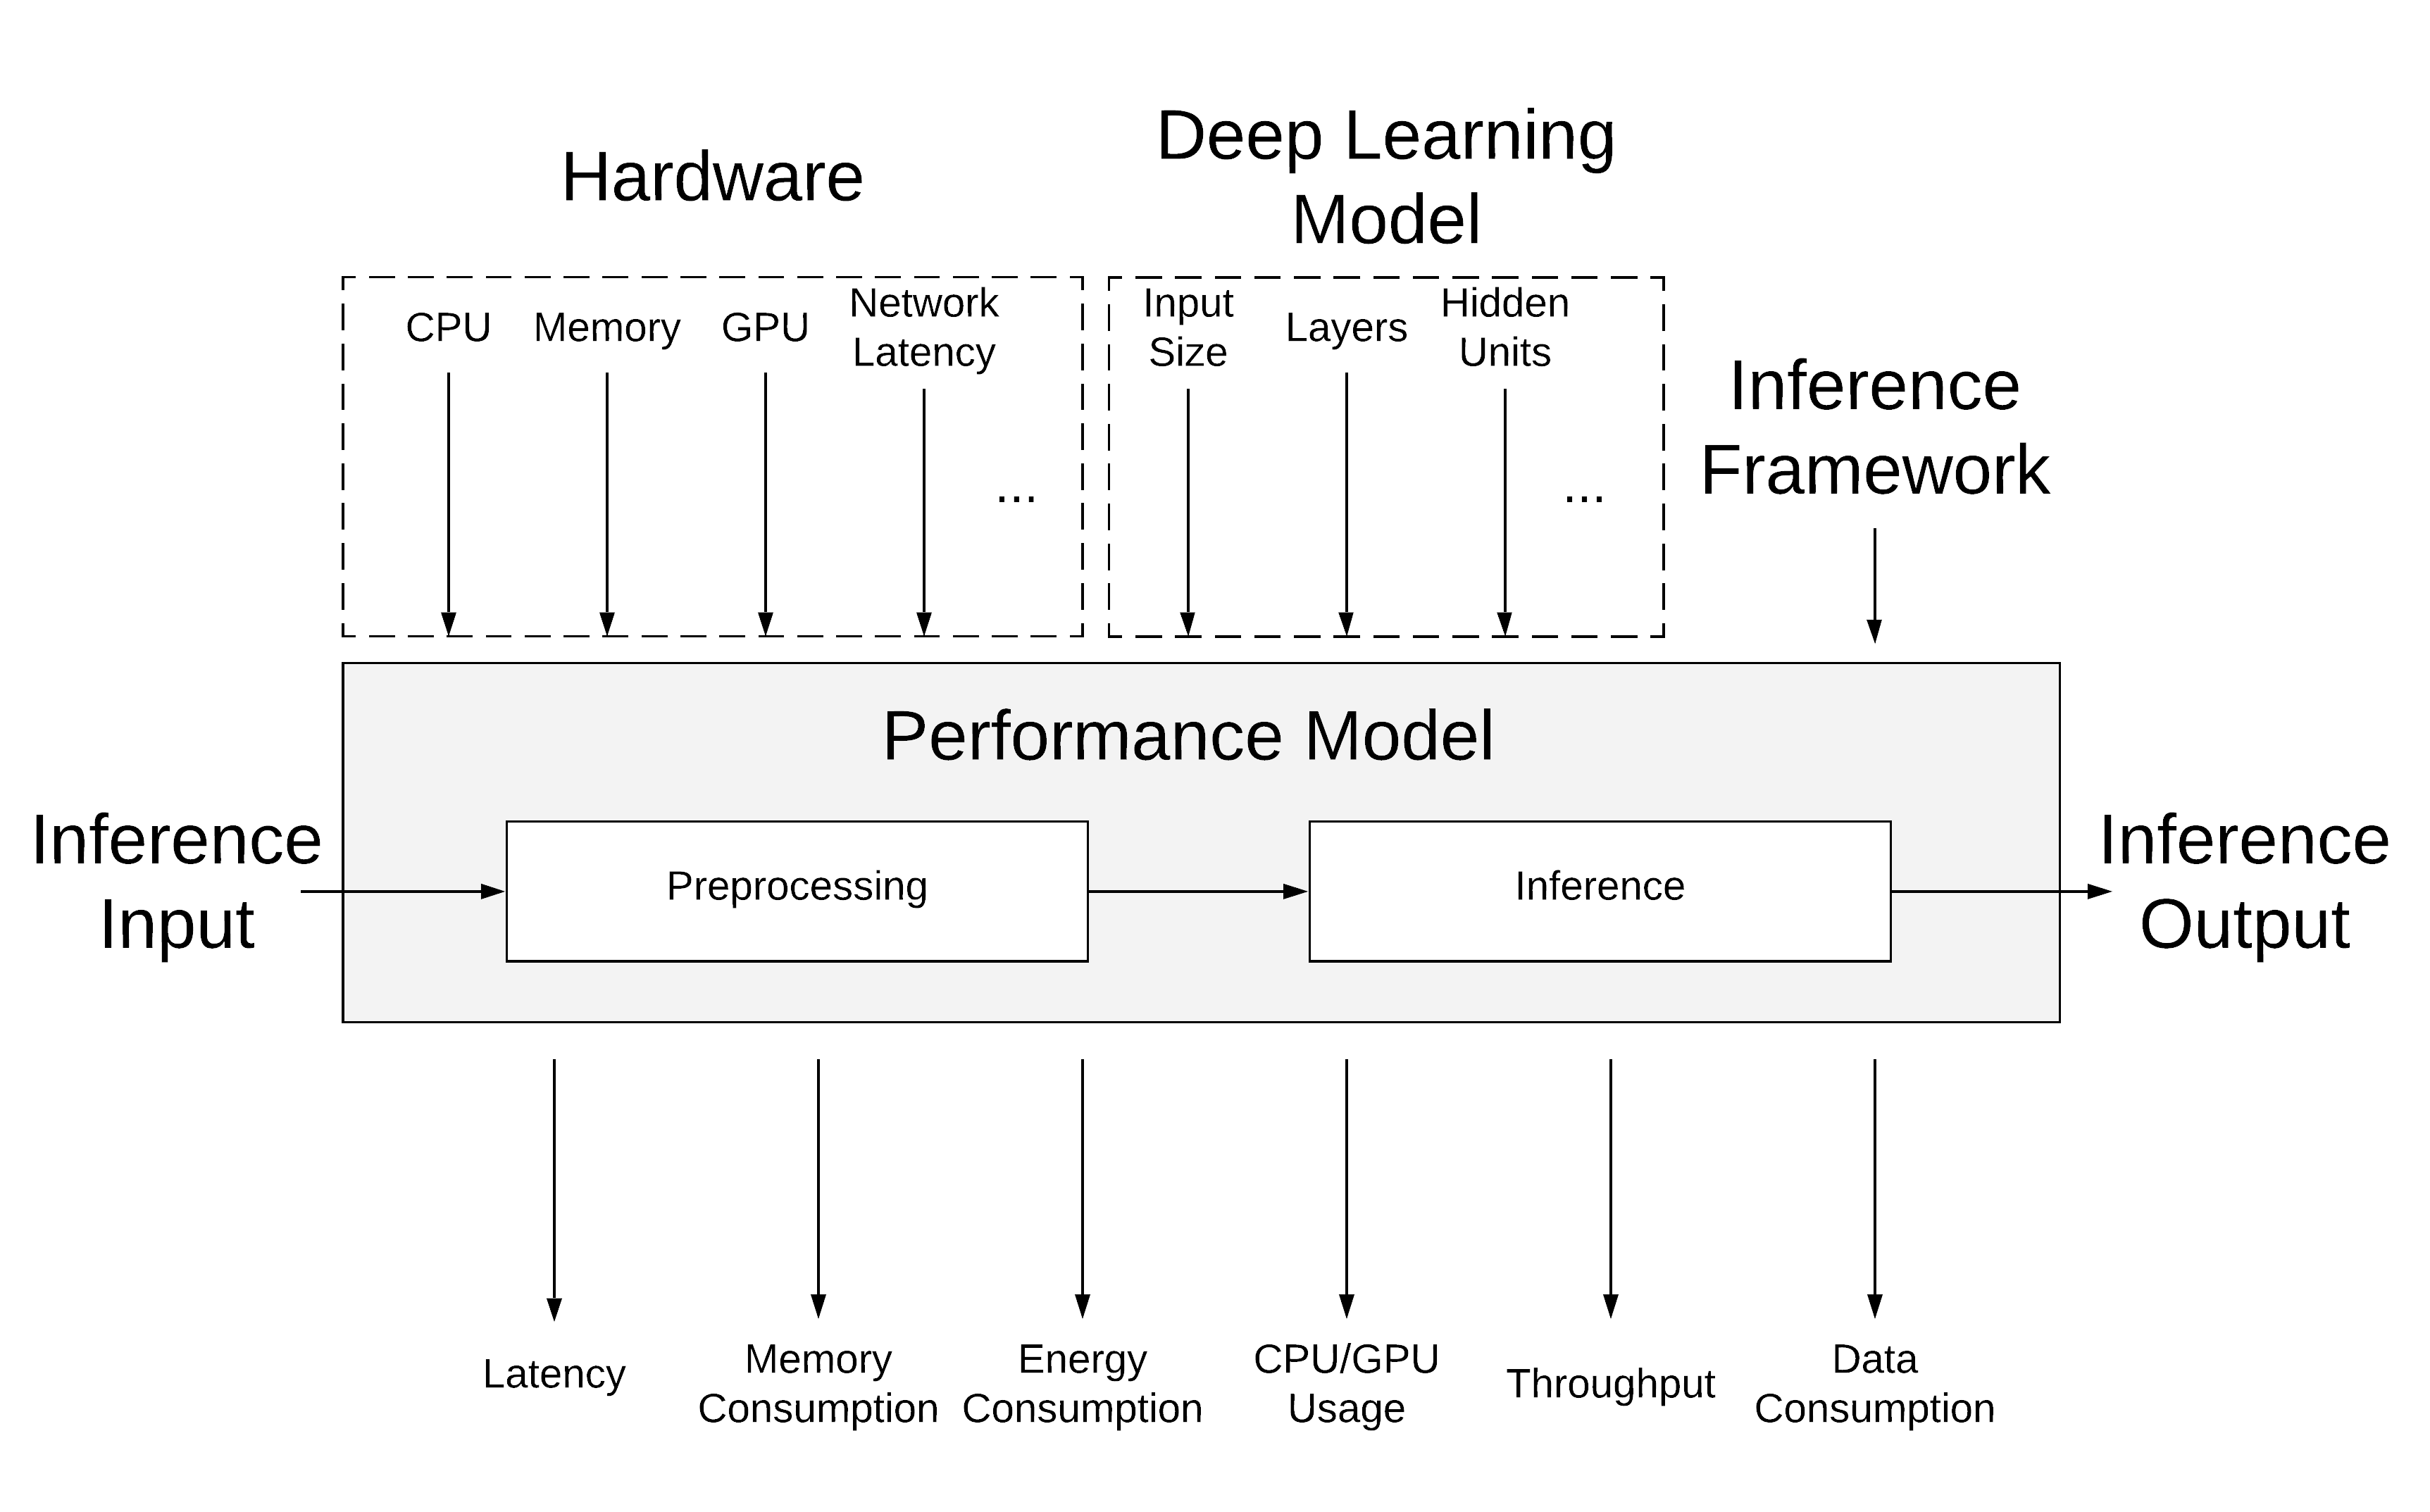
\includegraphics[width=0.99\textwidth]{./Bilder/PerformanceModel.png}
\caption{Performance Model with factors influencing the inference performance and the for the inference performance essential performance metrics}
\label{fig:perfmodel}
\end{figure}



To get the model output for a given model input two steps are needed. The first one is the preprocessing step and transforms a given input into the format that is required by the deep learning model. Only then the actual inference operation can be performed to obtain the model output. Therefore the preprocessing takes a vital part in the general inference process and should be included in the performance model.

\section{Performance Metrics}
\label{chap:metrics}
Several metrics are important to measure the performance of the preprocessing and the inference steps. For the most of the following metrics we break down each metric into two sub-measurements, one for the preprocessing  and the other for the inference part.

Except for data consumption, which is the only metric exclusive for cloud inference, because data is sent to a remote server, all metrics are relevant for both edge and cloud inference.
While accuracy is one of the most critical metrics for neural networks, it is only affected by the characteristics of the model and not by the deployment environment. Therefore we do not focus on accuracy in this thesis.

Note that we only measure the impact on inference/preprocessing on the resources on the edge devices, not the usage on the cloud-backend itself, as this theses focuses on optimal selection for real-time AI applications on edge devices.
\subsubsection{Latency}
Latencies are a essential to determine the performance, since AI application often need predictions in real-time, resulting in the need of low latencies.
The time needed to transform the original input to a shape fit for feeding into the deep learning model is called $Latency_{preprocessing}$.
%%WALL CLOCK TIME ADD HERE
$Latency_{inference}$ describes the time needed from requesting a prediction from a deep learning model given an specific input until getting the prediction.
The latency needed to perform both preprocessing and inference for a given input is called $Latency_{total}$.

For cloud inference, where network communication has to be done between a client (edge) and a server (cloud-backend), the network latency is an additional factor to the inference performance.
Therefore we split $Latency_{inference}$ in two sub metrics, $Latency_{network}$ and $Latency_{server}$, which together sum up to $Latency_{inference}$.
While $Latency_{server}$ denotes the time consumed by the cloud-backend to perform the inference on the given input, $Latency_{network}$ describes the time needed to send the inference input to the server and receive the prediction from the server.
\subsubsection{Throughput}
In order to accomplish realtime AI a certain level of throughput is essential. Therefore the number of predictions per second is a valuable metric. 
Since preprocessing is a vital part of the inference process, the throughput impact caused by preprocessed is also of interest.

Therefore we differentiate between three types of throughput: $Throughput_{preprocessing}$, $Throughput_{inference}$ and $Throughput_{total}$.
$Throughput_{total}$ is the throughput of the preprocessing and inference latencies combined.



\subsubsection{Energy Consumption}
$Energy_{preprocessing}$ and $Energy_{inference}$, which describe the amount of energy consumed during preprocessing and inference, are particular important for mobile edge devices, since they often are powered by batteries with a limited lifespan. If the preprocessing or inference process consumes too much energy, the application using the model is not viable.


\subsubsection{CPU/GPU Usage}
Since the preprocessing/inference operations are most of the time not the only processes running on a system and other processes need to run simultaneously, the usages of CPU ($CPU_{inference}$, $CPU_{preprocessing}$) and GPU ($GPU_{inference}$, $GPU_{preprocessing}$) or other available accelerators are an important metric.
High usages would also indicate that performance would eventually be slowed down on devices with less CPU/GPU power.


\subsubsection{Memory Usage}
Similar to CPU usage, preprocessing and inference should not occupy the whole memory of the system or even demand more memory than the available memory. Therefore $Memory_{inference}$ and $Memory_{preprocessing}$ are of interest.
%\subsubsection{GPU Usage}
%If a GPU or an another accelerator is available their usage is of interest.

\subsubsection{Data Consumption}
$Data_{transmitted}$ and $Data_{received}$ are only relevant for cloud inference, as a request has to be sent to a remote server and the according response with prediction has to be sent back to the client. A high data consumption could slow down the inference latency significantly if the up- and downstream of the network connection is too slow. 

This is in particular important for the case where the input data for the model is preprocessed on the cloud, because the input data is often resized to a smaller shape during preprocessing. Therefore cloud preprocessing increases the amount of data that needs to be transmitted to the server. For slow network connections this could result in higher inference latencies.

%%Add table here?


\section{Workload}
\begin{itemize}
    \item 3 image classification models
    \item one large, one small, one optimized
\end{itemize}
\section{Infrastructure}

\section{Benchmark System}


\section{Decision Model}
\begin{figure}[H]
\centering
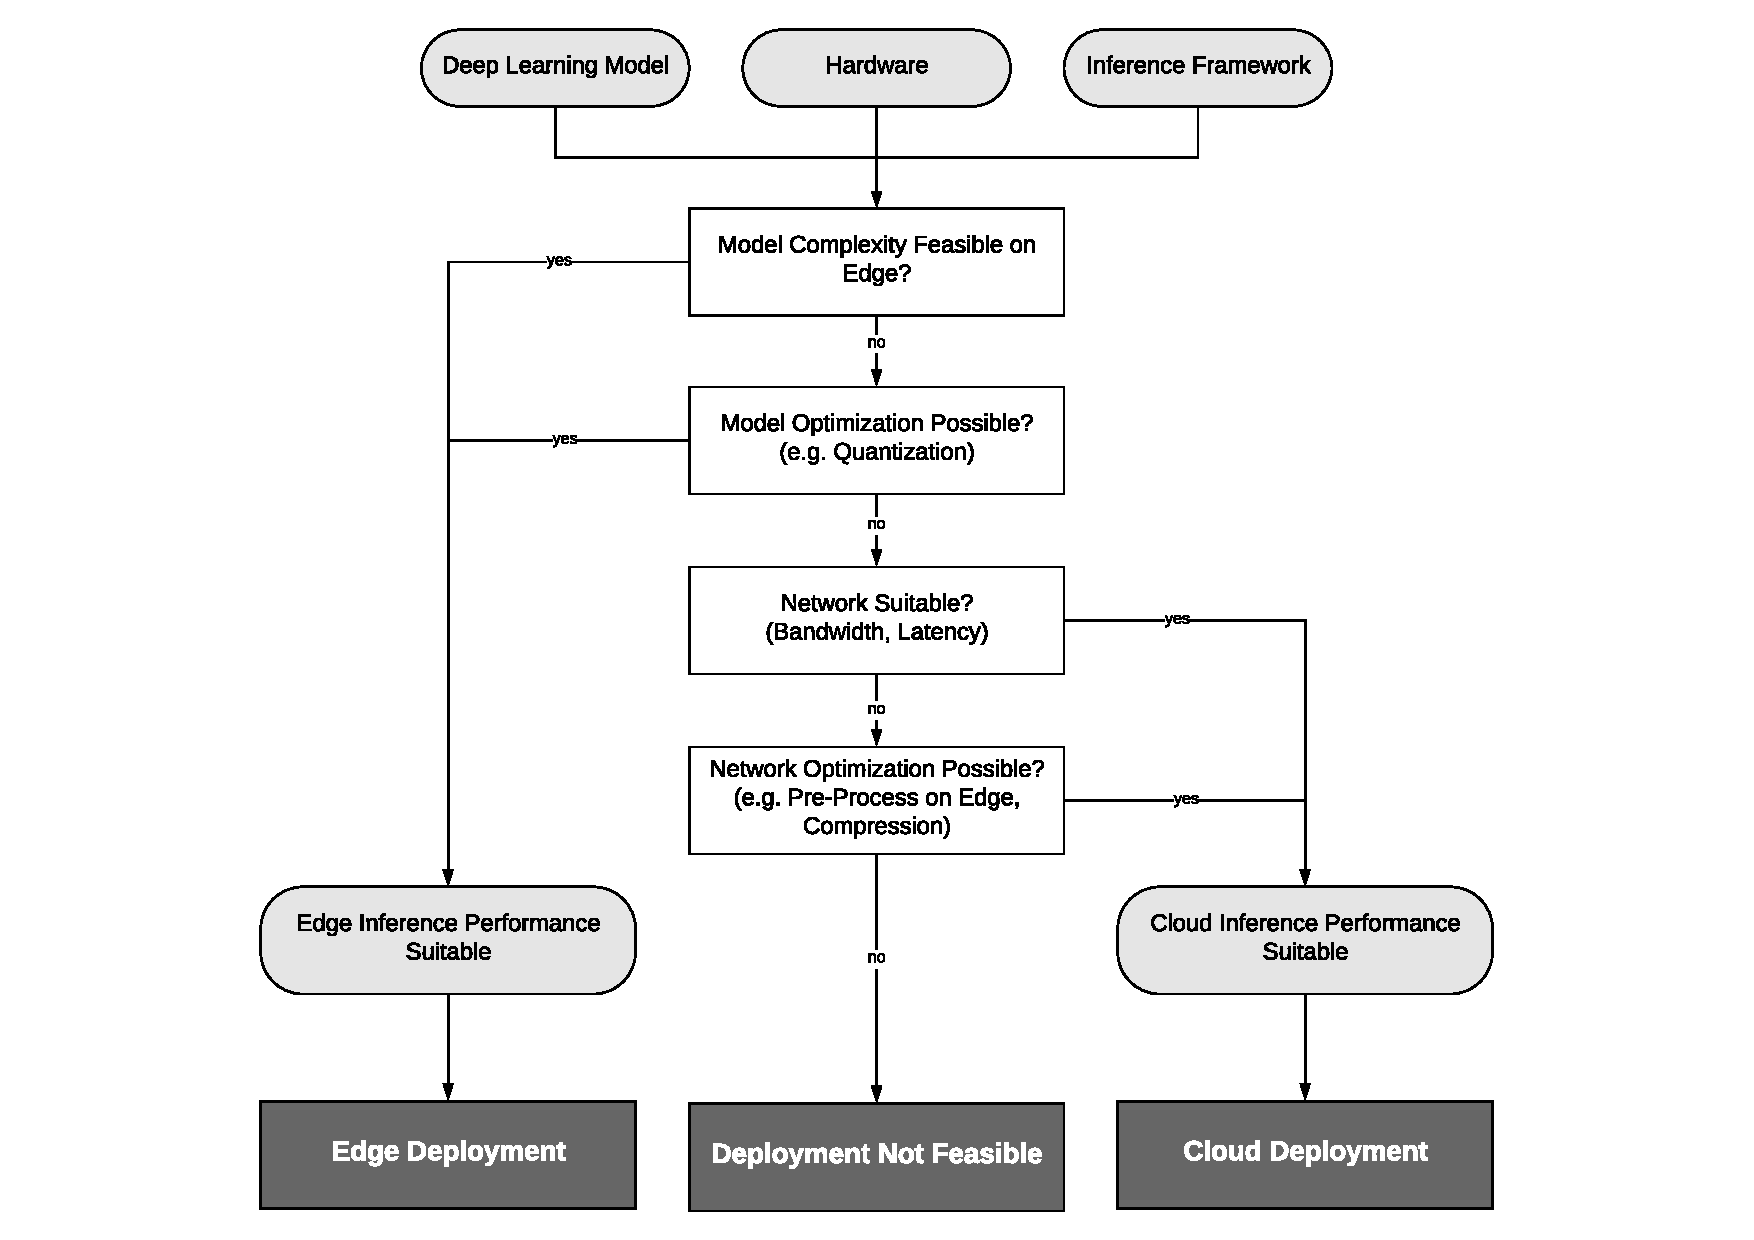
\includegraphics[width=0.99\textwidth]{./Bilder/DecisionModel.pdf}
\caption{Decision Model for optimal deployment selection}
\label{fig:DecisionModel}
\end{figure}


%%%%%%%%%%%%%%%%%%%%%%%%%%
%This section presented the factors influencing the performance of cloud and edge inference and the for the performance significant metrics.
%To model the relation between these factors and metrics, we perform experiments on both edge and cloud inference using state of the art hardware, model and framework components. The setup and the result of these experiments are covered in the next section.
\endinput 